\documentclass[a4paper, parskip=half]{scrartcl}
%\documentclass[a4paper, parskip=half]{scrartcl}
\usepackage[utf8]{inputenc}
\usepackage[T1]{fontenc}
\usepackage[english, ngerman]{babel}
%\usepackage{libertine}
\usepackage{xstring}
\usepackage{amssymb,amstext,amsmath}
\usepackage{graphicx}
\usepackage{sectsty}
\usepackage{multirow}
\usepackage{dsfont}
\usepackage{amsfonts}
\usepackage{graphics}
\usepackage{float}
\usepackage{dsfont}
\usepackage[hidelinks]{hyperref}
\usepackage{caption}
\usepackage{ifthen}
\usepackage[table]{xcolor}
\usepackage{booktabs}

\newcommand{\myMail}[1]{\href{mailto:#1}{#1}}

\newcommand{\myImage}[3][\textwidth]{
  \begin{center}
    \begin{minipage}{\linewidth}
      \centering 
      \makebox[0cm]{\includegraphics[width=#1]{#2}}
      \ifthenelse{ \equal{#3}{}} {
      
      } {
        \captionof{figure}{#3}
        %% \label{#3}
      }
    \end{minipage}
   
  \end{center}
}

\newcommand{\myTitlepage}{%
\begin{titlepage}
  \begin{center}
    \vspace{5cm}
    \huge\bfseries
    \myTitle
    \vspace{1cm}

    \large\normalfont von

    \bigskip
    \textbf{\myAuthor}

    \myDate

    \vspace{1cm}
    
    \large\normalfont
    Versuchsdurchführung am

    \textbf{\exDate}
    \vspace{1cm}
    
    Dozent

    \textbf{\exDoc}
    
    
    \myImage[10cm]{\myTitleImage}{}
  \end{center}
  \vfill
  \enlargethispage{2cm}
  \parbox[t]{0.55\textwidth}{%
   \myTitleLeft
  }
  \parbox[t]{0.45\textwidth}{\raggedleft%
    \myTitleRight
  }
\end{titlepage}
}

\newcommand{\mySecRef}[1]{%
  \hyperref[sec:#1]{Punkt-}\ref{sec:#1}%
}

\usepackage[english]{babel}
\usepackage{array}
\usepackage{calc}
%% \usepackage[paperwidth=15cm, paperheight=20cm]{geometry}

\newcommand{\myPackage}[1]{%
  \textit{#1}-Paket%
}

\newcommand{\myFormat}[1]{%
  \textit{#1}%
}

\newcommand{\myPath}[1]{%
  \textit{#1}%
}

\newcommand{\myTitle}{Ba 10: Scanning tunneling microscope}
\newcommand{\myAuthor}{Artem Gerassimoff, Alexander Heinisch, Dominik Wille}
\newcommand{\myDate}{\today}
\newcommand{\exDate}{02/05/2013 10am-2pm}
\newcommand{\exDoc}{Benjamin Heinrich}
\newcommand{\myTitleImage}{}
\newcommand{\myTitleLeft}{%
   \textbf{Freie Universität Berlin}\\
   Departement of physics\\
   Physikalisches Fortgeschrittenenpraktikum%
}
\newcommand{\myTitleRight}{%
 \textbf{Contact information:}\\
  \myMail{dominik.wille@fu-berlin.de} \\
  \myMail{matthias.heinisch@gmx.de} \\
  \myMail{art.geras@gmail.com}
}

\begin{document}
\begin{titlepage}
\begin{center}
    \vspace{5cm}
    \huge\bfseries
    \myTitle
    \vspace{1cm}

    \large\normalfont by

    \bigskip
    \textbf{\myAuthor}

    \myDate

    \vspace{1cm}
    
    \large\normalfont
    experiment execution on

    \textbf{\exDate}
    \vspace{1cm}
    
    docent

    \textbf{\exDoc}
    
    
  \end{center}
  \vfill
  \enlargethispage{2cm}
  \parbox[t]{0.55\textwidth}{%
   \myTitleLeft
  }
  \parbox[t]{0.45\textwidth}{\raggedleft%
    \myTitleRight
}
\end{titlepage}
\tableofcontents
\newpage
\section{Introduction}
The \textbf{Scanning tunneling microscope} short STM is a powerful method to determine information about the structure of soild bodies in the atomic scale. In this protocol  the stm will be introduced briefly with an example experimental observation of graphite.

\section{The principle of the Scanning tunneling microscope}
The principle of the STM is based on the quantum mechanical tunneling effect. In this case a cunducting needle is used to scan the surface of a cundicting body's surface. The needle should never hit the body but it should be so close to it ($<10 \mathring{\text{A}}$) so that there is notable tunneling current of electrons from the needle to the body. Therefore a electrical Potential from the needle to the body is needed in this experminent it will be in the $\text{mV}$-scale.

\subsection{Theoretical description}
\subsubsection{Quantum tunneling}
In quantum mechanics every particle's properties are described by a so called wave function $\psi$. Moreover classical properties like 
position and momentum are described statisally only which has far-reaching consequences for observations in the atomic scale.

One of the most common consequences is the eponymous \textit{quantum tunneling} which is derived from the fact that particles can
 pass potential barriers even with higher potential energies as their own kinetic energy, with some propability.

In first approximation the potential barrier can often be described as a rectangle.

\myImage[10cm]{img/tunnel}{Sketch of a particle stream tunneling through a barrier\cite{proto}}

As shown in the Sketch the wave function decreases in the barrier and the amplitude after the barrier is way smaller than before the barrier. The propabiltity that a particle tunnels through the barrier is given by:

\begin{align}
T &= \frac{1}{1 + \frac{V_0^2}{4E(V_0-E)}\sinh^2(2\kappa a)} \\
\text{with}\;\;\;\; \kappa &= \sqrt{\frac{2m}{\hbar^2}(V_0-E)}
\end{align}

Generally the tunneling current $I_t$ is proportional to the chance an electron overcomes the energy barrier given by the Work function.
\begin{align}
  I_t \propto V_t \cdot e^{-c \cdot \sqrt{\phi} \cdot s}
\end{align}
The wave-function of electrons in the solid body should fulfill the boundady condition that it is zero at the surface of the body. Moreover the wave-function of electrons in the body can be discriped as
\begin{align}
\psi = \psi_0 \cdot e^{-\chi z}
\end{align}
Where $\chi$ is discribes how fast the wave function decreases which usually depends on the used material and has the largest values close to the fermi temperature. 

\subsection{Piezoelectric plates}
The aim is to get a 3-dimensional image of the surface, so it's needed to vary the position the position of the needle in the atomic scale. It is obvious that every mechanical adjustment would have way to big inaccurencies. The common way to control the position of the needle accurately is to use piezoelectric plates.

Due to geometrical deformation of charges in the soild state body the plates deform if a volatge is applied.
\myImage[10cm]{img/piezo2}{Lead titanate $\mathrm{PbTiO_3}$ - Example piezo ceramic\cite{piezo2}}

\subsection{Graphite}
Graphite is an allotrope of carbon unlike diamond (which is an allotrope of carbon too) graphite's properties defines it as a conductor and a semimetal. Graphite has a layerd hexagonal structure. The atoms of every layer are places in the centers of the layer below.

\myImage[8cm]{img/graphite}{Crystal structure of graphite\cite{proto}}

\section{Experimental observation}
The STM requires a very accurate aquistation of the apperature therefore a all parts of the microscope are controlled by the nanotec\cite{nanotec} Software.

\subsection{The needle}
In principle one can say tha the tinier the tip of the neele the higher the resolution of the STM. There is no guarantee to get a good needly but it is obvious that the material should not corride. Moreover the material should not be exposed to the atmosphere for long to protect it from water etc. For investigation a platin-vanadium wire was cut while pulling it to produce the needle.
 
\subsection{Adjustment}
To get the STM to work he needle should never touch the sample but needs to get very close to it. The macroscopic adjustment was made with a micrometer screw controled by hand. To get an idea how close the needle already is there is a USB-camera. The final adjustment was made by a step motor connected to the sofware for controlling the  micrometer screw. The software did basically repeating the following process until there is a noteable tunneling current measured:
\begin{enumerate}
\item extend the piezo-plates
\item run in the piezo-plates
\item move forward the step motor
\end{enumerate}

\subsection{Scanning modes}
To get an image of the sample the x- and y-position of the needle is varied. Information about the surface of the smaple can be derived in different modes. The  most important modes are: 
\subsubsection{constant current}
In the constant current mode the height of the needle is varied so that the tunneling current keeps constant.
\subsubsection{constant height}
The z-position of the needle keeps constant and the information is derived from the tuneling current.

\section{Measurement}
\The resolution respectively the height of the needle above the sample is set indirectly via voltage and tunneling current. For higher voltages the distance from the needle to the sample becomes smaller for same current. For higher current the distace becomes smaller for same voltage. 
\subsection{full view}
To get an idea how the near landscape of the graphite surface looks like a scan of a $20\times20 \text{nm}$ sequence was made.
\myImage[10cm]{img/full_view}{$20\times20 \text{nm}$ sequence of a graphite surface}

\subsection{Edges}
To determine the height of edges a smaller sequence was recorded, the height can be derived from the profile of a route perpendicular to the edge.
\newpage
\begin{center}
\begin{tabular}{>{\centering\arraybackslash}m{2in} >{\centering\arraybackslash}m{2in} >{\centering\arraybackslash}m{1in}}
Image \\(line marks profile route) & Profile & edge heights \\\hline
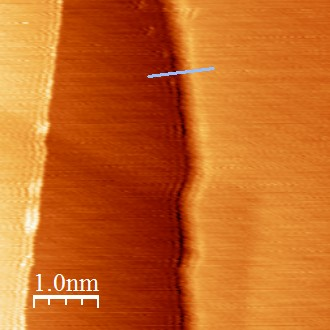
\includegraphics[width=3cm]{img/1} & 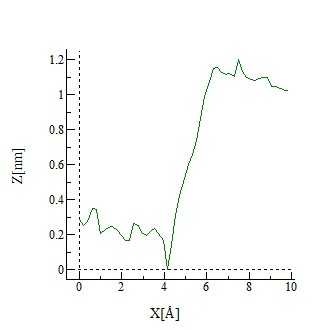
\includegraphics[width=3cm]{img/1_profile.jpg} & 1100 pm \\
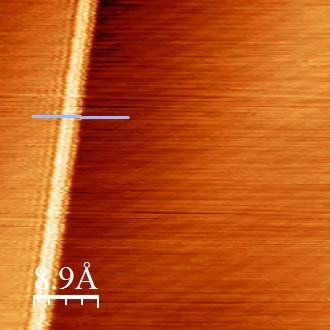
\includegraphics[width=3cm]{img/2} & 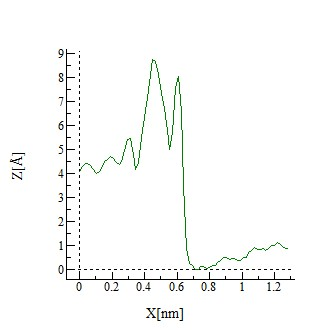
\includegraphics[width=3cm]{img/2_profile.jpg} & 350 pm, 700 pm  \\
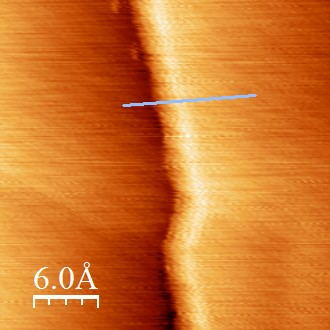
\includegraphics[width=3cm]{img/3} & 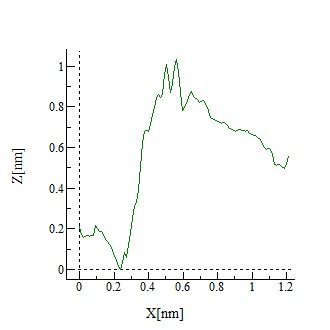
\includegraphics[width=3cm]{img/3_profile.jpg} & 900 pm \\
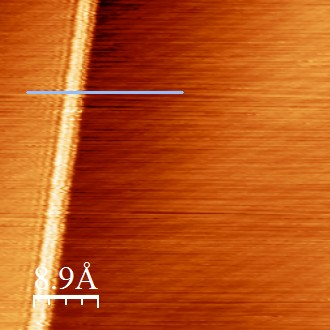
\includegraphics[width=3cm]{img/4} & 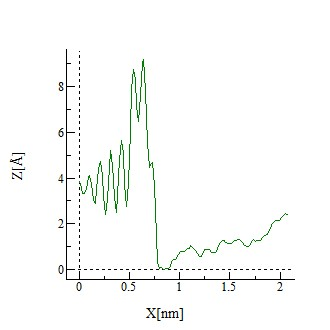
\includegraphics[width=3cm]{img/4_profile.jpg} & 350 pm, 400 pm \\
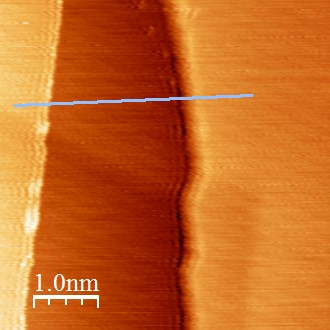
\includegraphics[width=3cm]{img/5} & 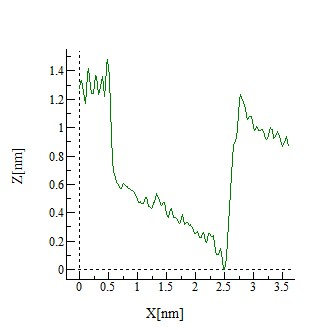
\includegraphics[width=3cm]{img/5_profile.jpg} & 700 pm, 1100 pm\\
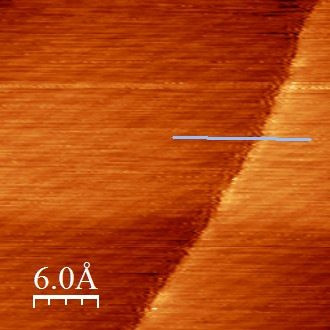
\includegraphics[width=3cm]{img/6} & 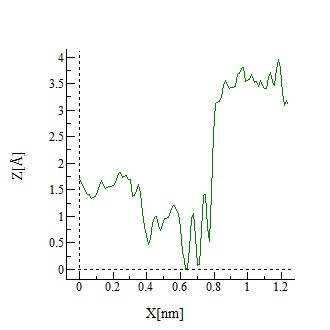
\includegraphics[width=3cm]{img/6_profile.jpg} & 300 pm \\
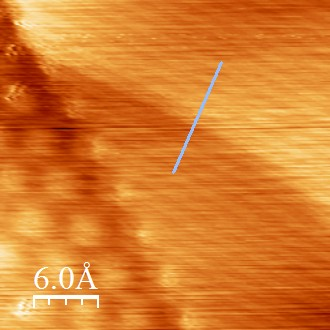
\includegraphics[width=3cm]{img/7} & 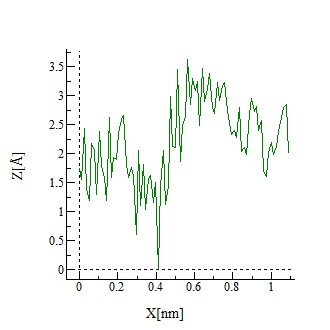
\includegraphics[width=3cm]{img/7_profile.jpg} & 150 pm
\end{tabular}
\end{center}
\newpage
\subsection{Data evaluation}
\myImage[10cm]{data/data}{summary of measured edge heights}
The height of a graphite layer is round about $335 \text{pm}$. It is clear that we have a lack of data to determine the height exactly but one can see that there is a accrual of points around multiples of $350 \text{pm}$ which are marked in the figure above. The deviation could be caused by a unperfect calibration of the experiment which would not be so unusual.

\subsection{Moiré pattern}
Due to lucky circumstances we had a special atomic makro structure, a so called moiré pattern. Such moire patterns appear when two otre more structured layers are twisted a little. To evaluate the structure the fourier 2D-transformation in the software was used.
\begin{center}
\begin{tabular}{>{\centering\arraybackslash}m{2in} >{\centering\arraybackslash}m{2in}}
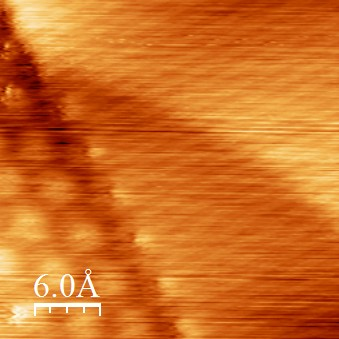
\includegraphics[width=5cm]{img/moire_0} & original image \\
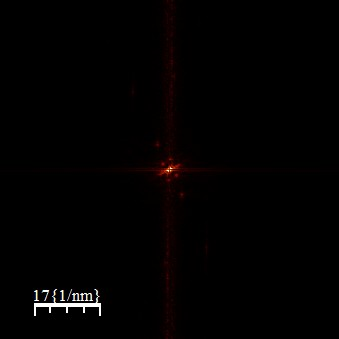
\includegraphics[width=5cm]{img/moire_fft} & fourier transformated \\
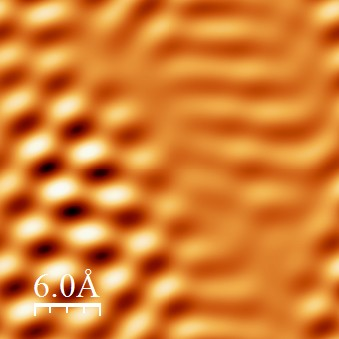
\includegraphics[width=5cm]{img/moire_1} & inverse fourier transformated of selected $k \approx \frac{1}{500 \text{pm}}$
\end{tabular}
\end{center}
The angular between those two layers can be calculated as:
\begin{align}
\alpha = 2 \cdot \arcsin\left( \frac{a_1 \cdot k}{2} \right) \approx 16,32^\circ
\end{align}

\section{Conclusion}
Eventhough we did not reached a resolution to detremine single atoms, the experiment was very successful! It was a very nice experience to seesuch small structures and how similar it looks like compared to makroscopic structures like mountains or valleys. Moreover we can verify the littreture value for the distance of two graphite layers and even determine a angular of two layers using a given atmoic distance of $142 \text{pm}}.   
\begin{thebibliography}{999}
\bibitem{piezo2} Taken from \url{http://en.wikipedia.org/wiki/Piezoelectricity}
\bibitem{nanotec} \url{http://www.nanotec.es/products/wsxm/}
\bibitem{proto} Taken from \url{http://www.weblars.de/downloads/Versuch\%20K122.pdf}

\end{thebibliography}
\end{document}
